% Copyright 2004 by Till Tantau <tantau@users.sourceforge.net>.
%
% In principle, this file can be redistributed and/or modified under
% the terms of the GNU Public License, version 2.
%
% However, this file is supposed to be a template to be modified
% for your own needs. For this reason, if you use this file as a
% template and not specifically distribute it as part of a another
% package/program, I grant the extra permission to freely copy and
% modify this file as you see fit and even to delete this copyright
% notice. 

\documentclass[aspectratio=169]{beamer}
%\documentclass{beamer}

\setbeamersize{text margin left=10mm, text margin right=10mm}

\defbeamertemplate{headline}{my header}{%
\vskip1pt%
\makebox[0pt][l]{\,\insertshortauthor}%
\hspace*{\fill}\insertshorttitle/\insertshortsubtitle\hspace*{\fill}%
\llap{\insertpagenumber/\insertpresentationendpage\,}
}
\setbeamertemplate{headline}[my header]

\usepackage{graphicx}
\usepackage{soul}
\usepackage{tkz-euclide}
\usetikzlibrary{calc}
\usepackage[]{algorithm2e}
\usepackage{changepage}
\usepackage{amssymb}
\usepackage{xcolor}
\usepackage{mathtools}
\usepackage{tcolorbox}
\usepackage{tikz}
\usetikzlibrary{arrows}
\usepackage{textcomp}
\usetikzlibrary{shapes}
\usepackage{tikz-3dplot}
\usepackage{tkz-euclide}
\usepackage{circuitikz}
\usepackage{pgfplots}
\pgfplotsset{width=7cm,compat=1.8}
\usetikzlibrary{positioning}
\usepackage[tikz]{bclogo}
\presetkeys{bclogo}{
ombre=false,
epBord=0,
couleur = black!10!white,
couleurBord = red,
arrondi = 0.1,
logo=,
}{}
% \usepackage[math]{cellspace}
% \cellspacetoplimit 4pt
% \cellspacebottomlimit 4pt
%\usetikzlibrary{arrows.meta}
% sqare of half axes
\newcommand{\asa}{3}
\newcommand{\bsa}{1}
\newcommand{\csa}{0.25}
% view angle
\tdplotsetmaincoords{70}{135}

%\setbeamertemplate{itemize items}{-}

%\usepackage{helvet}
\usefonttheme{professionalfonts} % using non standard fonts for beamer
%\usefonttheme{serif} % default family is serif
%\usepackage{fontspec}
%\setmainfont{Liberation Serif}

% There are many different themes available for Beamer. A comprehensive
% list with examples is given here:
% http://deic.uab.es/~iblanes/beamer_gallery/index_by_theme.html
% You can uncomment the themes below if you would like to use a different
% one:
%\usetheme{AnnArbor}
%\usetheme{Antibes}
%\usetheme{Bergen}
%\usetheme{Berkeley}
%\usetheme{Berlin}
%\usetheme{Boadilla}
%\usetheme{boxes}
%\usetheme{CambridgeUS}
%\usetheme{Copenhagen}
%\usetheme{Darmstadt}
%\usetheme{default}
%\usetheme{Frankfurt}
%\usetheme{Goettingen}
%\usetheme{Hannover}
%\usetheme{Ilmenau}
%\usetheme{JuanLesPins}
%\usetheme{Luebeck}
%\usetheme{Madrid}
%\usetheme{Malmoe}
%\usetheme{Marburg}
%\usetheme{Montpellier}
%\usetheme{PaloAlto}
%\usetheme{Pittsburgh}
%\usetheme{Rochester}
%\usetheme{Singapore}
%\usetheme{Szeged}
%\usetheme{Warsaw}

% Definition of blocks:
\tikzset{%
  block/.style    = {draw, thick, rectangle, minimum height = 3em,
    minimum width = 3em},
  sum/.style      = {draw, circle, node distance = 2cm}, % Adder
  input/.style    = {coordinate}, % Input
  output/.style   = {coordinate} % Output
}
% Defining string as labels of certain blocks.
\newcommand{\suma}{\Large$+$}
\newcommand{\inte}{$\displaystyle \int$}
\newcommand{\derv}{\huge$\frac{d}{dt}$}

\def\mf{\ensuremath\mathbf}
\def\mb{\ensuremath\mathbb}
\def\lp{\ensuremath\left(}
\def\rp{\ensuremath\right)}
\def\lv{\ensuremath\left\lvert}
\def\rv{\ensuremath\right\rvert}
\def\lV{\ensuremath\left\lVert}
\def\rV{\ensuremath\right\rVert}
\def\lc{\ensuremath\left\{}
\def\rc{\ensuremath\right\}}
\def\ls{\ensuremath\left[}
\def\rs{\ensuremath\right]}
\def\bmx{\ensuremath\begin{bmatrix*}[r]}
\def\emx{\ensuremath\end{bmatrix*}}
\def\bmxc{\ensuremath\begin{bmatrix*}[c]}
\def\t{\lp t\rp}
\def\k{\ls k\rs}


\newcommand{\demoex}[2]{\onslide<#1->\begin{color}{black!60} #2 \end{color}}
\newcommand{\demoexc}[3]{\onslide<#1->\begin{color}{#2} #3 \end{color}}
\newcommand{\anim}[3]{\onslide<#1->{\begin{color}{#2!60} #3 \end{color}}}
\newcommand{\ct}[1]{\lp #1\rp}
\newcommand{\dt}[1]{\ls #1\rs}
\newcommand{\cols}[2]{\begin{columns}[#1] #2 \end{columns}}
\newcommand{\col}[2]{\begin{column}{#1} #2 \end{column}}


% \newenvironment{rcases}
% {\left.\begin{aligned}}
% {\end{aligned}\right\rbrace}


\title{Linear Systems}

% A subtitle is optional and this may be deleted
\subtitle{Solution of LDS}

\author{Sivakumar Balasubramanian}
% - Give the names in the same order as the appear in the paper.
% - Use the \inst{?} command only if the authors have different
%   affiliation.

\institute[Christian Medical College] % (optional, but mostly needed)
{
  \inst{}%
  Department of Bioengineering\\
  Christian Medical College, Bagayam\\
  Vellore 632002
}
% - Use the \inst command only if there are several affiliations.
% - Keep it simple, no one is interested in your street address.

\date{}
% - Either use conference name or its abbreviation.
% - Not really informative to the audience, more for people (including
%   yourself) who are reading the slides online

\subject{Lecture notes on linear systems}
% This is only inserted into the PDF information catalog. Can be left
% out. 

% If you have a file called "university-logo-filename.xxx", where xxx
% is a graphic format that can be processed by latex or pdflatex,
% resp., then you can add a logo as follows:

% \pgfdeclareimage[height=0.5cm]{university-logo}{university-logo-filename}
% \logo{\pgfuseimage{university-logo}}

% Delete this, if you do not want the table of contents to pop up at
% the beginning of each subsection:
\AtBeginSubsection[]
{
  \begin{frame}<beamer>{Outline}
    \tableofcontents[currentsection,currentsubsection]
  \end{frame}
}

% Let's get started
\begin{document}

\pgfplotsset{
  compat=1.8,
  colormap={whitered}{color(0cm)=(white); color(1cm)=(orange!75!red)}
}

\begin{frame}
  \titlepage
\end{frame}


\begin{frame}[t]{State space representation of LDS}
\begin{itemize}
    \item A state space representation of a LTI system takes the following form,
    \[ \dot{\mf{x}}\ct{t} = \mf{A}\mf{x}\ct{t} + \mf{B}\mf{u}\ct{t} \]
    \[ \mf{y}\ct{t} = \mf{C}\mf{x}\ct{t} + \mf{D}\mf{u}\ct{t} \]

    \item Obtaining the solution to the above equations can be posed as the following prolbem,
    \[ \begin{rcases}
    \text{Determine:  }  \mf{x}\ct{t}, \, \mf{y}\ct{t} \,\,\, \forall t \geq 0 \\
    \text{Given:  }  \mf{u}\ct{t}, \, \forall t \geq 0 \text{ and } \mf{x}\ct{0^{-}} \\
    \end{rcases}
    \]

    \item We first solve the state equation to obtain $\mf{x}\ct{t}$, which is then used to obtain $\mf{y}\ct{t}$.

    \item Because the system is linear, we can separate the solution into zero-input and zero-state solutions.
\end{itemize}
\end{frame}


\begin{frame}[t]{Zero-input solution for $\mf{x}\ct{t}$}
\begin{itemize}
    \item \textbf{Zero-Input Solution}: We will start by assuming $\mf{u}\ct{t} = \mf{0}$.
    \[ \dot{\mf{x}}\ct{t} = \mf{A}\mf{x}\ct{t} \]

    \item For the scalar case, $\dot{x}\ct{t} = ax\ct{t}$, we know the solution to be the following, $x\ct{t} = e^{at}x\ct{0^-}$.

    \item A similar approach works for the vector case. Let us assume to the solution to zero-input state equation to be of the form, $\mf{x}\ct{t} = e^{t\mf{A}}\mf{x}\ct{0^-}$. 
\end{itemize}
\end{frame}


\begin{frame}[t]{Zero-input solution for $\mf{x}\ct{t}$}
\begin{itemize}
    \item What is $e^{t\mf{A}}$? Functions of matrices are often defined to have properties consistent with that of their scalar coutnerparts. 
     \[ e^{t\mf{A}} = \mf{I} + t\mf{A} + \frac{1}{2!}t^2\mf{A}^2 + \ldots = \sum_{k=0}^{\infty} \frac{1}{k!}t^k\mf{A}^k \implies \frac{d}{dt}e^{t\mf{A}} = \mf{A}e^{t\mf{A}} \]

   \item Thus, $\mf{x}\ct{t} = e^{t\mf{A}}\mf{x}\ct{0^-}$ is the zero-input solution.
\end{itemize}
\end{frame}


\begin{frame}[t]{$f\lp\mf{A}\rp$: functions of square matrices}
\begin{itemize}
    \item How do we evaluate $e^{t\mf{A}}$? We do not need to evaluate the infinite series.

    \begin{bclogo}{Cayley-Hamilton Theorem}
    Every square matrix $\mf{A} \in \mb{R}^{n \times n}$ satisfies it own characteristic equation $p\lp \lambda \rp = 0$, i.e. $p\lp\mf{A}\rp = \mf{0}$.
    \[ p\lp\mf{A}\rp = \mf{A}^n + a_1\mf{A}^{n-1} + a_2\mf{A}^{n-2} + \ldots + a_n\mf{I} = \mf{0} \]
    \end{bclogo}
\end{itemize}
\end{frame}


\begin{frame}[t]{$f\lp\mf{A}\rp$: functions of square matrices}
\begin{itemize}
    \item Consider a analytic function, $f\lp x\rp = \sum_{k=0}^\infty a_kx^k$, and a matrix $\mf{A} \in \mb{R}^{n \times n}$ with characteristic polynomial $p\lp x\rp$. Then,
    \[ f\lp x\rp = q\lp x\rp p\lp x\rp + r\lp x\rp \]
    where, $q\lp x\rp$ and $r\lp x\rp$ are the quotient and reminder polynomials, respectively, and $r\lp x\rp = c_0 + c_1x + c_2x^2 + \ldots + c_{n-1}x^{n-1}$.

    Since $p\lp \mf{A}\rp = \mf{0}$, we have $f\lp \mf{A}\rp = r\lp \mf{A}\rp = \sum_{k=0}^{n-1}c_k\mf{A}^k$. Determining $c_k$s will allow us to calulate $f\lp \mf{A}\rp$.
\end{itemize}
\end{frame}


\begin{frame}[t]{$f\lp\mf{A}\rp$: functions of square matrices}
\begin{itemize}
    \item If $\mf{A}$ has $n$ distinct eigenvalues, $c_k$s solved through the $n$ equations, $f\lp \lambda_i\rp = q\lp\lambda_i\rp p\lp\lambda_i\rp + r\lp \lambda_i\rp = r\lp \lambda_i\rp$.

    \item For repeated eigenvalues, we will need the following,
    \[ \frac{d^{m-1}}{dx^{m-1}}f\lp x\rp\biggr\rvert_{x=\lambda_i} = \frac{d^{m-1}}{dx^{m-1}}r\lp x\rp\biggr\rvert_{x=\lambda_i} \]
    
    \item For a diagonalizable matrix, $e^{t\mf{A}} = \mf{X}e^{t\mf{\Lambda}}\mf{X}^{-1}$, with $e^{t\mf{\Lambda}} = \text{diag}\lp e^{\lambda_1t} \ldots e^{\lambda_nt}\rp$.

    \item For non-diagonalizable matrix we have,
    $e^{t\mf{A}} = \mf{X}\bmxc e^{t\mf{J}_1} &  &  &\\
          & e^{t\mf{J}_2} &  &\\
          & & \ddots &\\
          &  &  & e^{t\mf{J}_k}\emx\mf{X}^{-1}$
\end{itemize}
\end{frame}


\begin{frame}[t]{$f\lp\mf{A}\rp$: functions of square matrices}
Evaluate $e^{t\mf{A}}$ for the following $\mf{A}$: (a) $\bmx 1 & 2 \\ 0 & 2\emx$; (b) $\bmx 1 & 2 \\ 0 & 1\emx$; (c) $\bmx 0 & 1\\ -1 & 0\emx$
\end{frame}


\begin{frame}[t]{$f\lp\mf{A}\rp$: functions of square matrices}
Evaluate $e^{t\mf{J}}$ for $\mf{J}$ with $GM=1$: (a) $AM=2$; (b) $AM=3$; (c) $AM=n$.
\end{frame}


\begin{frame}[t]{Laplace transform approach to zero-input response $\mf{x}\ct{t}$}
\begin{itemize}
    \item Taking the Unilateral Laplace transform of the zero-input state equation, 
    \[ s\mf{x}_{\mathcal{L}}\ct{s} - \mf{x}\ct{0^-} = \mf{A}\mf{x}_{\mathcal{L}}\ct{s} \]
    where, $\mf{x}_{\mathcal{L}}\ct{s} = \bmx X_1\ct{s} & X_2\ct{s} \ldots X_n\ct{s}\emx^T$, where $x_i\ct{t} \xleftrightarrow{\mathcal{L}} X_i\ct{s}$.

    \[ \lp s\mf{I} - \mf{A}\rp\mf{x}_{\mathcal{L}}\ct{s} = \mf{x}\ct{0^-} \implies \mf{x}_{\mathcal{L}}\ct{s} = \lp s\mf{I} - \mf{A}\rp^{-1}\mf{x}\ct{0^-}\]

    \[ \implies \mf{x}\ct{t} = \mathcal{L}^{-1}\lc\lp s\mf{I} - \mf{A}\rp^{-1}\rc\mf{x}\ct{0^-}\]

    \item Using the analogy from the scalar case, we could guess that $\mf{x}\ct{t} = e^{t\mf{A}}\mf{x}\ct{0^-}$. One can obtain the same solution by first finding the $\lp s\mf{I} - \mf{A}\rp^{-1}$ and taking the inverse Laplace of each entry of this matrix. 
\end{itemize}
\end{frame}


\begin{frame}[t]{Laplace transform approach to zero-input response $\mf{x}\ct{t}$}
Find $\mf{x}\ct{t}$ for $t \geq 0$: $\dot{\mf{x}}\ct{t} = \bmx 1 & 2 \\ 0 & 2\emx \mf{x}\ct{t}$.
\end{frame}


\begin{frame}[t]{Properties of $e^{t\mf{A}}$}
\begin{itemize}
    \item The columns of $e^{t\mf{A}} = \bmx \mf{a}_{1}\ct{t} & \mf{a}_{2}\ct{t} & \ldots \mf{a}_{n}\ct{t}\emx$ represent the solutions to different initial conditions, i.e. $\mf{x}\ct{t} = \mf{a}_i\ct{t} = e^{t\mf{A}}\mf{e}_i$.
    \[ \mf{x}\ct{t} = e^{t\mf{A}}\mf{x}\ct{0^-} = e^{t\mf{A}}\sum_{i=1}^n x_i\ct{0^-}\mf{e}_i = \sum_{i=1}^n x_i\ct{0^-}\mf{a}_i \]

    \item If we know the response of a system to a set of $n$ linearly independent initial conditions. Let $\mf{X}\ct{t}$ represent the matrix whose columns are the solutions to the different initial conditions, then for any given intial condition $\mf{x}\ct{0^-}$, we have the solution,
    \[ \mf{x}\ct{t} = \mf{X}\ct{t}\lp \mf{X}\ct{0^-}\rp^{-1}\mf{x}\ct{0^-} \] 
\end{itemize}
\end{frame}


\begin{frame}[t]{Properties of $e^{t\mf{A}}$}
\begin{itemize}
    \item For any arbitrary initial time $\tau$, instead of $0$, we can still use the exponential formula to find out the solution,
    \[ \mf{x}\ct{t} = e^{\lp t - \tau\rp\mf{A}}\mf{x}\ct{\tau} \]

    \item $e^{t\mf{A}}$ is called the \textit{state transition matrix}, which takes the state at any given time to its value $t$ seconds forward in time.
\end{itemize}
\end{frame}


\begin{frame}[t]{Diagonalization of a linear system}
\begin{itemize}
    \item Consider the case where, $\mf{A}$ is diagonalizable. Let $\lc\lambda_i, \mf{v}_i\rc_{i=1}^n$ be the eigenpairs of $\mf{A}$. Then, $\mf{A} = \mf{V}\mf{\Lambda}\mf{V}^{-1}$, and we could write the zero-input state equation as,
    \[ \dot{\mf{x}}\ct{t} = \mf{V}\mf{\Lambda}\mf{V}^{-1}\mf{x}\ct{t} \xrightarrow[]{\tilde{\mf{x}}\ct{t} = \mf{V}^{-1}\mf{x}\ct{t}} \dot{\tilde{\mf{x}}}\ct{t} = \mf{\Lambda}\tilde{\mf{x}}\ct{t} \]

    The set of coupled first order differential equations are decoupled by this transforamtion.

    \item The individual states of $\tilde{\mf{x}}\ct{t}$ evolve independently of each other.
    $$\tilde{\mf{x}}\ct{t} = e^{t\mf{\Lambda}}\tilde{\mf{x}}\ct{0^-} = \bmx 
    e^{\lambda_1 t} & & & \\
     & e^{\lambda_2 t} & & \\
     & & \ddots & \\
     & & & e^{\lambda_n t}
    \emx \tilde{\mf{x}}\ct{0^-}$$
\end{itemize}
\end{frame}


\begin{frame}[t]{Diagonalization of a linear system}
\begin{itemize}
    \item An arbitrary initial state $\mf{x}\ct{0^-} = \sum_{i=1}^{n}\alpha_i\mf{v}_i$ evolves as follows,
    \[ \mf{x}\ct{t} = \alpha_1e^{\lambda_1t}\mf{v}_1 + \alpha_2e^{\lambda_2t}\mf{v}_2 + \ldots + \alpha_ne^{\lambda_nt}\mf{v}_n\]
\end{itemize}
\end{frame}


\begin{frame}[t]{Diagonalization of a linear system}
When $\mf{A}$ is not diagonalizable: $\mf{A} = \mf{V}\mf{J}\mf{V}^{-1} \implies$ $\dot{\tilde{\mf{x}}}\ct{t} = \mf{J}\tilde{\mf{x}}\ct{t}$.
\[ \tilde{\mf{x}}\ct{t} = e^{t\mf{J}}\tilde{\mf{x}}\ct{0^-} = \bmx 
e^{t\mf{J}_1} & & \\
 & \ddots & \\
 & & e^{t\mf{J}_k}
\emx \tilde{\mf{x}}\ct{0^-} \]

Consider $\mf{A} = \mf{V}\bmx \lambda & 1 \\ 0 & \lambda\emx\mf{V}^{-1} \implies \dot{\tilde{\mf{x}}}\ct{t} = \bmx \lambda & 1 \\ 0 & \lambda\emx\tilde{\mf{x}}\ct{t}$ 
\[ \begin{split}
\dot{\tilde{x}}_1\ct{t} &= \lambda\tilde{x}_1\ct{t} + \tilde{x}_2\ct{t}\\
\dot{\tilde{x}}_2\ct{t} &= \lambda\tilde{x}_2\ct{t}
\end{split}  \]

We do not have complete decoupling as in the case where $\mf{A}$ was diagonalizable.
\end{frame}


\begin{frame}[t]{Diagonalization of a linear system}
The exponential of a Jordan block has terms $e^{\lambda t}$, $te^{\lambda t}$, $te^{\lambda t}$, $\ldots$
\[ e^{t\mf{J}_1} = e^{\lambda_1 t}\bmxc 
1 & t & \frac{t^2}{2!} & \ldots & \frac{t^n}{n!}\\ 
0 & 1 & t & \ldots & \frac{t^{n-1}}{\lp n-1\rp!}\\
0 & 0 & 1 & \ldots & \frac{t^{n-2}}{\lp n-2\rp!}\\
\vdots & \vdots & \vdots & \ddots & \vdots\\
0 & 0 & 0 & \ldots & 1
\emx \]

Thus, 
\[ \begin{split}
\tilde{x}_1\ct{t} &= \tilde{x}_1\ct{0^-}e^{\lambda t} + \tilde{x}_2\ct{0^-}te^{\lambda t}\\
\tilde{x}_2\ct{t} &= \tilde{x}_2\ct{0^-}e^{\lambda t}
\end{split} \]
\end{frame}


\begin{frame}[t]{Diagonalization of a linear system}
\begin{columns}[t]
\begin{column}{0.3\textwidth}
\[ \dot{\mf{x}}\ct{t} = \bmx 1  & 2\\0 & 2\emx \mf{x}\ct{t} \]
\begin{center}
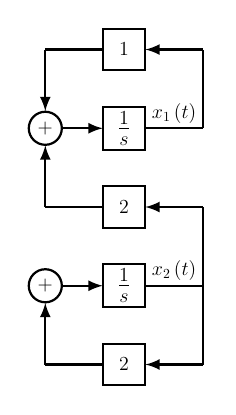
\begin{tikzpicture}[scale=0.5, transform shape, thick, node distance=2cm]
\draw
    node [input, name=input1] {} 
    node [sum, right of=input1] (suma1) {\suma}
    node [block, right of=suma1] (inte1) {{\huge $\frac{1}{s}$}}
    node [output, right of=inte1, name=output1] {}    
    node [block, above of=inte1] (scale11) {{\Large $1$}}
    node [input, right of=scale11, name=temp11] {}
    node [output, above of=suma1, name=temp12] {}

    node [block, below of=inte1] (scale12) {{\Large $2$}}
    node [input, left of=scale12, name=temp31] {}
    node [input, right of=scale12, name=temp32] {}

    node [sum, below of=temp31] (suma2) {\suma}
    node [input, left of=suma2, name=input2] {}
    node [block, right of=suma2] (inte2) {{\huge $\frac{1}{s}$}}
    node [output, right of=inte2, name=output2] {}    
    node [block, below of=inte2] (scale22) {{\Large $2$}}
    node [input, right of=scale22, name=temp21] {}
    node [output, below of=suma2, name=temp22] {};

    % \draw[-latex](input1) -- node {}(suma1);
    \draw[-latex](suma1) -- node {} (inte1);
    \draw[-](inte1) -- node [above] {{\Large $x_1\ct{t}$}}(output1);
    \draw[-](output1) -- node {}(temp11);
    \draw[-latex](temp11) -- node {}(scale11);
    \draw[-](scale11) -- node {}(temp12);
    \draw[-latex](temp12) -- node {}(suma1);

    % \draw[-latex](input2) -- node {}(suma2);
    \draw[-latex](suma2) -- node {} (inte2);
    \draw[-](inte2) -- node [above] {{\Large $x_2\ct{t}$}}(output2);
    \draw[-](output2) -- node {}(temp21);
    \draw[-latex](temp21) -- node {}(scale22);
    \draw[-](scale22) -- node {}(temp22);
    \draw[-latex](temp22) -- node {}(suma2);
    % \draw[-](output) -- node {}(suma1);

    \draw[-](output2) -- node {}(temp32);
    \draw[-latex](temp32) -- node {}(scale12);
    \draw[-](scale12) -- node {}(temp31);
    \draw[-latex](temp31) -- node {}(suma1);
\end{tikzpicture}
\end{center}
\end{column}

\begin{column}{0.3\textwidth}
\end{column}
\begin{column}{0.4\textwidth}
\end{column}
\end{columns}
\end{frame}


\begin{frame}[t]{Diagonalization of a linear system}
\begin{columns}[t]
\begin{column}{0.3\textwidth}
When $\mf{A}$ is diagonalizable.
\[ \dot{\tilde{\mf{x}}}\ct{t} = \bmx 1  & 0\\0 & 2\emx \tilde{\mf{x}}\ct{t} \]

\begin{center}
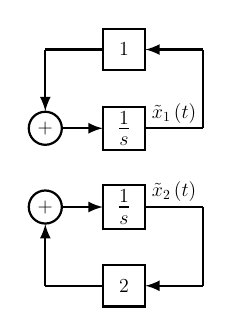
\begin{tikzpicture}[scale=0.5, transform shape, thick, node distance=2cm]
\draw
    node [input, name=input1] {} 
    node [sum, right of=input1] (suma1) {\suma}
    node [block, right of=suma1] (inte1) {{\huge $\frac{1}{s}$}}
    node [output, right of=inte1, name=output1] {}    
    node [block, above of=inte1] (scale11) {{\Large $1$}}
    node [input, right of=scale11, name=temp11] {}
    node [output, above of=suma1, name=temp12] {}

    node [sum, below of=suma1] (suma2) {\suma}
    node [input, left of=suma2, name=input2] {}
    node [block, right of=suma2] (inte2) {{\huge $\frac{1}{s}$}}
    node [output, right of=inte2, name=output2] {}    
    node [block, below of=inte2] (scale22) {{\Large $2$}}
    node [input, right of=scale22, name=temp21] {}
    node [output, below of=suma2, name=temp22] {};

    % \draw[-latex](input1) -- node {}(suma1);
    \draw[-latex](suma1) -- node {} (inte1);
    \draw[-](inte1) -- node [above] {{\Large $\tilde{x}_1\ct{t}$}}(output1);
    \draw[-](output1) -- node {}(temp11);
    \draw[-latex](temp11) -- node {}(scale11);
    \draw[-](scale11) -- node {}(temp12);
    \draw[-latex](temp12) -- node {}(suma1);

    % \draw[-latex](input2) -- node {}(suma2);
    \draw[-latex](suma2) -- node {} (inte2);
    \draw[-](inte2) -- node [above] {{\Large $\tilde{x}_2\ct{t}$}}(output2);
    \draw[-](output2) -- node {}(temp21);
    \draw[-latex](temp21) -- node {}(scale22);
    \draw[-](scale22) -- node {}(temp22);
    \draw[-latex](temp22) -- node {}(suma2);
    % \draw[-](output) -- node {}(suma1);
\end{tikzpicture}
\end{center}
\end{column}

\begin{column}{0.3\textwidth}
\end{column}

\begin{column}{0.4\textwidth}
\end{column}
\end{columns}
\end{frame}


\begin{frame}[t]{Diagonalization of a linear system}
\begin{columns}[t]
\begin{column}{0.4\textwidth}
When $\mf{A}$ is not-diagonalizable.
\[ \dot{\tilde{\mf{x}}}\ct{t} = \bmx 1  & 1\\0 & 1\emx \tilde{\mf{x}}\ct{t} \]
\begin{center}
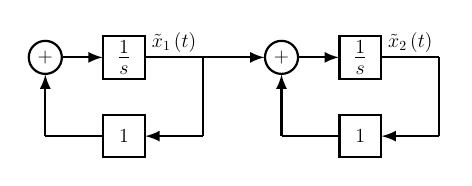
\begin{tikzpicture}[scale=0.5, transform shape, thick, node distance=2cm]
\draw
    node [input, name=input1] {} 
    node [sum, right of=input1] (suma1) {\suma}
    node [block, right of=suma1] (inte1) {{\huge $\frac{1}{s}$}}
    node [output, right of=inte1, name=output1] {}    
    node [block, below of=inte1] (scale11) {{\Large $1$}}
    node [input, right of=scale11, name=temp11] {}
    node [output, below of=suma1, name=temp12] {}

    % node [input, right of=output1, name=input2] {}
    node [sum, right of=output1] (suma2) {\suma}
    node [block, right of=suma2] (inte2) {{\huge $\frac{1}{s}$}}
    node [output, right of=inte2, name=output2] {}    
    node [block, below of=inte2] (scale22) {{\Large $1$}}
    node [input, right of=scale22, name=temp21] {}
    node [output, below of=suma2, name=temp22] {};

    % \draw[-latex](input1) -- node {}(suma1);
    \draw[-latex](suma1) -- node {} (inte1);
    \draw[-](inte1) -- node [above] {{\Large $\tilde{x}_1\ct{t}$}}(output1);
    \draw[-](output1) -- node {}(temp11);
    \draw[-latex](temp11) -- node {}(scale11);
    \draw[-](scale11) -- node {}(temp12);
    \draw[-latex](temp12) -- node {}(suma1);

    \draw[-latex](output1) -- node {}(suma2);
    \draw[-latex](suma2) -- node {} (inte2);
    \draw[-](inte2) -- node [above] {{\Large $\tilde{x}_2\ct{t}$}}(output2);
    \draw[-](output2) -- node {}(temp21);
    \draw[-latex](temp21) -- node {}(scale22);
    \draw[-](scale22) -- node {}(temp22);
    \draw[-latex](temp22) -- node {}(suma2);
\end{tikzpicture}
\end{center}
A Jordan block results in series of simple (scalar) first order blocks, where the output of a block acts as the input to another.
\end{column}

\begin{column}{0.3\textwidth}
\end{column}

\begin{column}{0.3\textwidth}
\end{column}
\end{columns}
\end{frame}


\begin{frame}[t]{Modes of a system}
\vspace{-0.5cm}
\[ \dot{\mf{x}}\ct{t} = \mf{A}\mf{x}\ct{t} \implies \mf{x}\ct{t} = \sum_{i=1}^n \alpha_ie^{\lambda_it}\mf{v}_i \]
\vspace{-0.5cm}

\begin{itemize}
    \item The eigvenvalues $\lc \lambda_i\rc_{i=1}^n$ of the system matrix $\mf{A}$ characterize the ``natural'' behavior of the system. These are called the \textit{modes of the system}.

    \item The modes are exclusively expressed when the system starts in some specific set of states. When the system starts in an arbitrary state, the  response contains a linear mixtute of these modes.
\end{itemize}
\end{frame}


\begin{frame}[t]{Modes of a system}
\vspace{-0.5cm}
\[ \dot{\mf{x}}\ct{t} = \mf{A}\mf{x}\ct{t} \implies \mf{x}\ct{t} = \sum_{i=1}^n \alpha_ie^{\lambda_it}\mf{v}_i \]
\vspace{-0.5cm}

\begin{itemize}
    \item \textbf{Dominant mode}: Determines the long-term behavior of the system. In the case of continuous-time systems, this would be the eigenvalue with the largest real part.

    \item If $\lambda_i$ is a dominant mode $\implies \lv \alpha_ie^{\lambda_it} \rv \gg \lv \alpha_je^{\lambda_jt} \rv, \forall j \neq i$ and $t > T$.

    This implies that after some time, the response almost only has that particular mode,
    \[ \mf{x}\ct{t} \approx \alpha_ie^{\lambda_i t}\mf{v}_i, \,\,\, \forall t > T \]

    \item \textbf{Subdominant mode}: These are the other modes of the system, and these essentially determine how fast the system moves to the dominant mode.
\end{itemize}
\end{frame}


\begin{frame}[t]{Modes of a system}
\cols{}{
    \col{0.5\textwidth}{
        {\small Consider the system, $\dot{\mf{x}}\ct{t} = \bmx -1 & 2 \\ 0 & -5\emx\mf{x}\ct{t}$. 
                
        $\textbf{Modes:} \begin{cases}
        \lambda_1 = -1, & \mf{v}_1 = \bmx 1 & 0\emx^T\\
        \lambda_2 = -5, & \mf{v}_2 = \bmx 1 & 2\emx^T
        \end{cases}$}
        \begin{center}
        \begin{tikzpicture}[scale=1.0]
            \node[anchor=south west,inner sep=0] at (0,0) {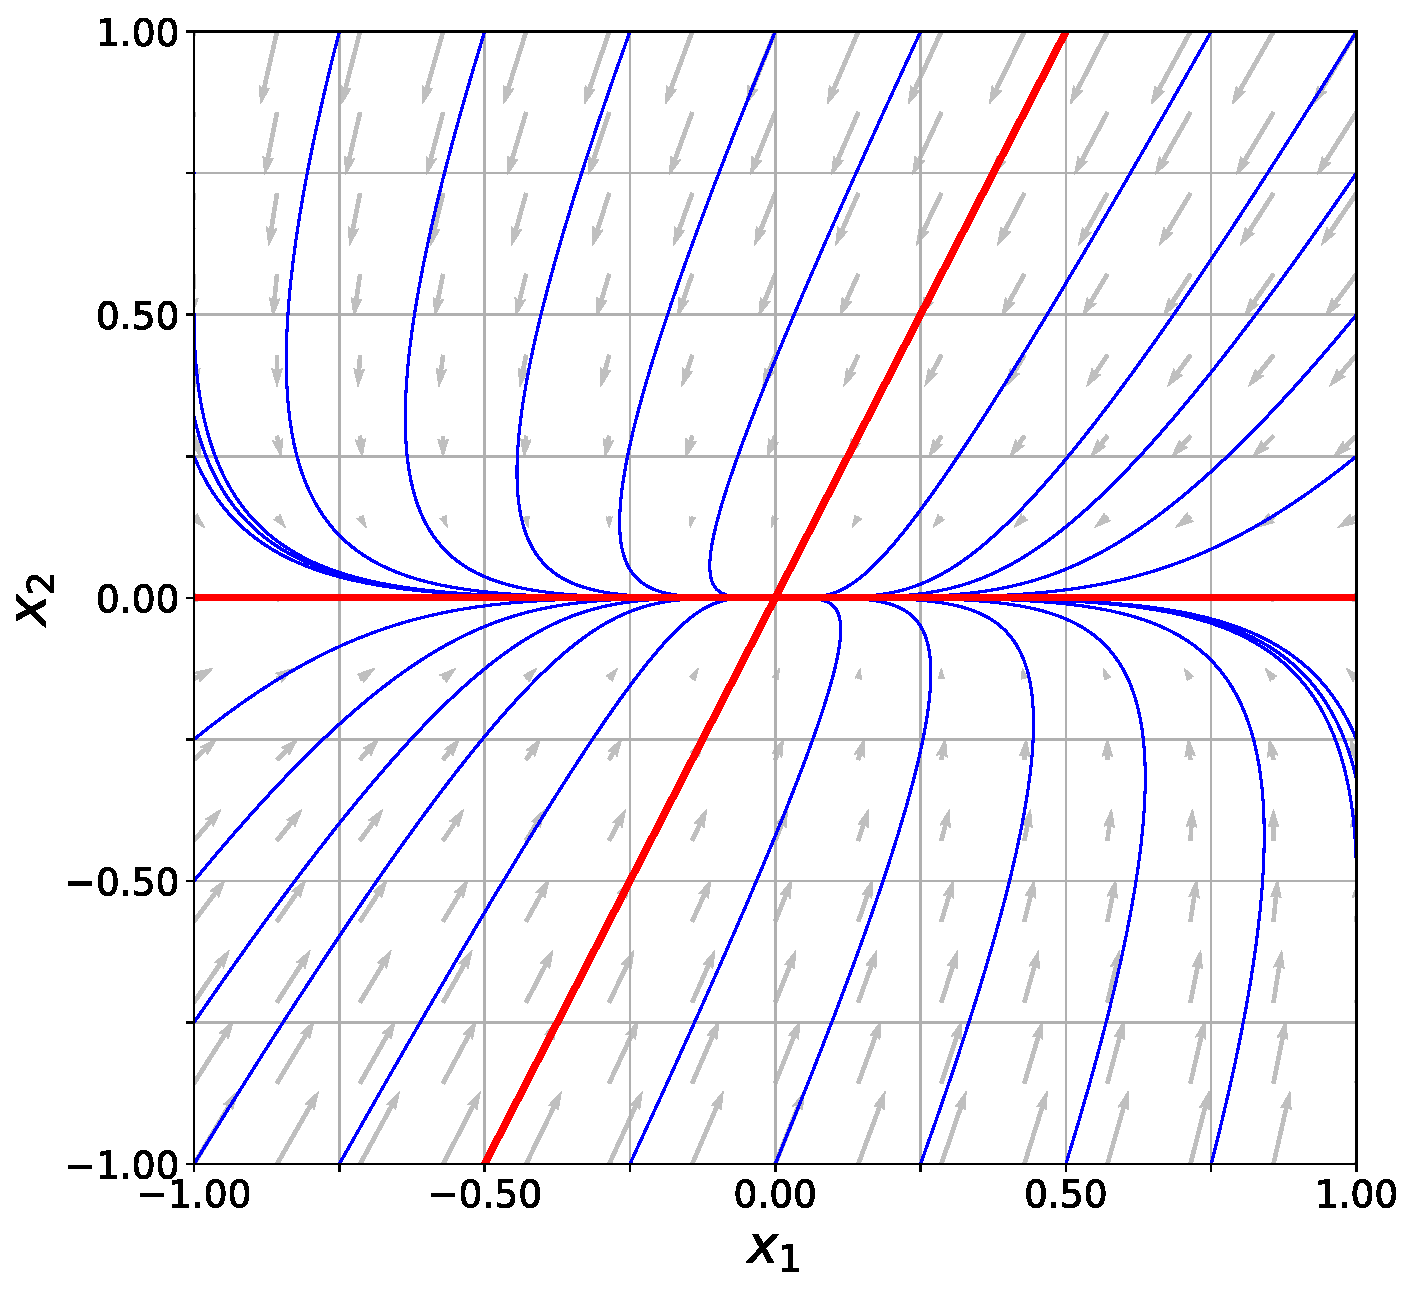
\includegraphics[width=0.7\textwidth]{img/modes.eps}};
            \draw[white, fill=white!20] (0.75,2.2) rectangle (1.15,2.6);
            \node[black] at (0.95, 2.4) {$\mf{v}_1$};
            \draw[white, fill=white!20] (1.6,0.5) rectangle (2.0,0.9);
            \node[black] at (1.8, 0.7) {$\mf{v}_2$};
        \end{tikzpicture}
        \end{center}
    }
    \col{0.5\textwidth}{
    Consider a system with modes: $\lp -1, \mf{v}_1 \rp$, $\lp -1, \mf{v}_2\rp$, $\lp -3, \mf{v}_3 \rp$, and $\lp -10, \mf{v}_4\rp$. What are the dominant modes? How does any arbitrary state evolve?
    }
}
\end{frame}


\begin{frame}[t]{Modes of a system}
Describe the state equation of a mass $M$ in free space. What are its modes?
\end{frame}


\begin{frame}[t]{Zero-solution for $\mf{x}\ct{t}$}
\begin{itemize}
    \item Let us now assume that the LTI system is relaxed when the input the applied to the system, i.e. $\mf{x}\ct{0^-} = \mf{0}$. The effect of the input $\mf{u}\ct{t}$ can be obtained by working in the Laplace domain,
    \[ \dot{\mf{x}}\ct{t} = \mf{A}\mf{x}\ct{t} + \mf{B}\mf{u}\ct{t} \implies \mf{x}_{\mathcal{L}}\ct{s} = \lp s\mf{I} - \mf{A}\rp^{-1}\mf{B}\mf{u}_{\mathcal{L}}\ct{s} \]

    Taking the inverse Laplace transform, we get,
    \[ \mf{x}\ct{t} = \int_{0}^{\infty} e^{\ct{t - \tau}\mf{A}}\mf{B}\mf{u}\ct{\tau}d\tau \]
\end{itemize}
\end{frame}


\begin{frame}[t]{Zero-solution for $\mf{x}\ct{t}$}
What do the columns of $e^{t\mf{A}}\mf{B}$ represent? What about the row of $e^{t\mf{A}}\mf{B}$? What about the $ij^{th}$ element of $e^{t\mf{A}}\mf{B}$?
\end{frame}


\begin{frame}[t]{Complete solution for $\mf{x}\ct{t}$ and $\mf{y}\ct{t}$}
\begin{itemize}
    \item The complete solution for the state equations is given by the following,
    \[ \mf{x}\ct{t} = e^{t\mf{A}}\mf{x}\ct{0^-} + \int_{0}^{\infty}e^{\ct{t - \tau}\mf{A}}\mf{B}\mf{u}\ct{\tau}d\tau \]

    \item The output of the system is given by,
    \[ \mf{y}\ct{t} = \mf{C}e^{t\mf{A}}\mf{x}\ct{0^-} + \int_{0}^{\infty}\mf{C}e^{\ct{t - \tau}\mf{A}}\mf{B}\mf{u}\ct{\tau}d\tau + \mf{D}\mf{u}\ct{t} = \mf{C}e^{t\mf{A}}\mf{x}\ct{0^-} + \int_{0}^{\infty}\mf{G}\ct{t - \tau}{u}\ct{\tau}d\tau \]

    where, $\mf{G}\ct{t} = \mf{C}e^{t\mf{A}}\mf{B} + \mf{D}\delta\ct{t}$ is the \textit{impulse response matrix} of the system. 

    \item The transfer function of the system is given by: $\mf{H}\ct{s} = \mf{C}\lp s\mf{I} - \mf{A}\rp^{-1}\mf{B} + \mf{D}$.
\end{itemize}
\end{frame}


\begin{frame}[t]{Complete solution for $\mf{x}\ct{t}$ and $\mf{y}\ct{t}$}
Find the impulse response matrix for $\mf{A} = \bmx 1 & 2\\0 & 1\emx$, $\mf{B} = \bmx 1 & -0.5\\1 & 1\emx$, $\mf{C} = \bmx 1 & 0\emx$, and $\mf{D} = 0$.
\end{frame}


\begin{frame}[t]{Complete solution for $\mf{x}\ct{t}$ and $\mf{y}\ct{t}$}
Find the expression for $\mf{y}\ct{t} = \bmx v_{C_1}\ct{t} & v_{R_2}\ct{t}\emx^T$ for the following system, such that $v_{C_1}\ct{0^-} = 1V$, $v_{C_2}\ct{0^-} = -0.5V$, $u_1\ct{t} = 1\ct{t}V$, and $R=1k\Omega, C=1mF$.
\vspace{-0.3cm}
\begin{center}
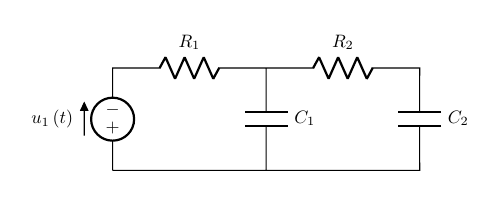
\begin{tikzpicture}[scale=0.65, transform shape]
\path (0,0) coordinate (ref_gnd);
\draw
  (ref_gnd) to[american voltage source=$u_1\lp t\rp$] ++(0,2)
            to[R=\(R_1\)] ++(3,0) 
            to[C=\(C_1\)] ++(0,-2) 
  -- (ref_gnd)
  (3,2) to[R=\(R_2\)] ++(3,0)
        to[C=\(C_2\)] ++(0,-2) 
  -- (ref_gnd);
\end{tikzpicture}
\end{center}
\end{frame}


\begin{frame}[t]{Solution for discrete-time LTI system}
\begin{itemize}
    \item \textbf{System equations}:
    \[ \mf{x}\dt{k+1} = \mf{A}\mf{x}\dt{k} + \mf{B}\mf{u}\dt{k} \]
    \[ \mf{y}\dt{k} = \mf{C}\mf{x}\dt{k} + \mf{D}\mf{u}\dt{k} \]

    \item \textbf{Zero-input solution}:
    $$\mf{x}\dt{k} = \mf{A}^k\mf{x}\dt{0}$$

    \item \textbf{Zero-state solution}:
    $$ \mf{x}\dt{k} = \sum_{l=0}^{k-1}\mf{A}^{k-l-1}\mf{B}\mf{u}\dt{l}$$
\end{itemize}
\end{frame}


\begin{frame}[t]{Solution for discrete-time LTI system}
\begin{itemize}
    \item \textbf{Complete solution}:
    $$\mf{x}\dt{k} = \mf{A}^k\mf{x}\dt{0} + \sum_{l=0}^{k-1}\mf{A}^{k-l-1}\mf{B}\mf{u}\dt{l}$$

    \item $\mf{A}^k$ is the \textit{state transition matrix} and $\mf{G}\dt{k} = \mf{A}^{k - 1}\mf{B}$ is the \textit{impulse response matrix}.
\end{itemize}
\end{frame}


\begin{frame}[t]{Solution for discrete-time LTI system}
\begin{itemize}
    \item We can approach this problem through the z-transform. Taking the unilateral z-transform of the state equation, 
    \[ z\mf{X}_{\mathcal{Z}}\ct{z} - z\mf{x}\ct{0} = \mf{A}\mf{X}_{\mathcal{Z}}\ct{z} + \mf{B}\mf{U}_{\mathcal{Z}}\ct{z} \]

    \[ \mf{X}_{\mathcal{Z}}\ct{z} = z\lp z\mf{I} - \mf{A}\rp^{-1}\mf{x}\dt{0} +  \lp z\mf{I} - \mf{A}\rp^{-1}\mf{B}\mf{U}_{\mathcal{Z}}\ct{z} \]
    
    The inverse z-tansform of this leads us to,
    $$\mf{x}\dt{k} = \mf{A}^k\mf{x}\dt{0} + \sum_{l=0}^{k-1}\mf{A}^{k-l-1}\mf{B}\mf{u}\dt{l}$$
\end{itemize}
\end{frame}


\begin{frame}[t]{Solution for discrete-time LTI system}
\begin{itemize}
    \item Output:
    $$ \mf{y}\dt{k} = \mf{C}\mf{A}^k\mf{x}\dt{0} + \sum_{l=0}^{k-1}\mf{C}\mf{A}^{k-l-1}\mf{B}\mf{u}\dt{l} + \mf{D}\mf{u}\dt{k} $$

    \item The transfer function of the system is, $\mf{H}\ct{z} = \mf{C}\lp z\mf{I} - \mf{A}\rp^{-1}\mf{B} + \mf{D}$
\end{itemize}
\end{frame}


\begin{frame}[t]{Diagonalization of a linear system}
\textbf{When $\mf{A}$ is diagonalizable}, then we have

\[ \mf{x}\dt{k + 1} = \mf{V}\mf{\Lambda}\mf{V}^{-1}\mf{x}\dt{k} \implies \tilde{\mf{x}}\dt{k + 1} = \mf{\Lambda}\tilde{\mf{x}}\dt{k} \]\vspace{-0.5cm}

where, $\tilde{\mf{x}}\dt{k} = \mf{V}^{-1}\mf{x}\dt{k}$.

\[ \tilde{\mf{x}}\dt{k} = \mf{\Lambda}^k\tilde{\mf{x}}\dt{0} = \bmx 
 \lambda_1^k & & & \\
 &  \lambda_2^k & & \\
 & & \ddots & \\
 & & &  \lambda_n^k
\emx \tilde{\mf{x}}\dt{0} \]

An arbitrary initial state $\mf{x}\dt{0} = \sum_{i=1}^{n}\alpha_i\mf{v}_i$ evolves as follows,
\[ \mf{x}\dt{k} = \alpha_1 \lambda_1^k\mf{v}_1 + \alpha_2 \lambda_2^k\mf{v}_2 + \ldots + \alpha_n \lambda_n^k\mf{v}_n\]
\end{frame}


\begin{frame}[t]{Diagonalization of a linear system}
\textbf{When $\mf{A}$ is not diagonalizable}, $\mf{A} = \mf{V}\mf{J}\mf{V}^{-1}$

\[ \tilde{\mf{x}}\dt{k+1} = \mf{J}\tilde{\mf{x}}\dt{k+1} \] \vspace{-0.8cm}

\[ \tilde{\mf{x}}\dt{k} = \mf{J}^k\tilde{\mf{x}}\dt{0} = \bmx 
 \mf{J}_1^k & & \\
 & \ddots & \\
 & &  \mf{J}_l^k
\emx \tilde{\mf{x}}\dt{0} \]
\end{frame}

\begin{frame}[t]{Diagonalization of a linear system}
Consider $\mf{A} = \mf{V}\bmx \lambda & 1 \\ 0 & \lambda\emx\mf{V}^{-1} \implies \tilde{\mf{x}}\dt{k+1} = \bmx \lambda & 1 \\ 0 & \lambda\emx\tilde{\mf{x}}\dt{k}$ \vspace{-0.25cm}
\[ \begin{split}
\tilde{x}_1\dt{k+1} &= \lambda\tilde{x}_1\dt{k} + \tilde{x}_2\dt{k}\\
\tilde{x}_2\dt{k+1} &= \lambda\tilde{x}_2\dt{k}
\end{split} \]\vspace{-0.75cm}

\[ \mf{J}^k = \lambda^k \bmxc 
1 & \frac{k!\lambda^{-1}}{\lp k-1\rp!1!} & \frac{k!\lambda^{-2}}{\lp k-2\rp! 2!} & \ldots & \frac{k!\lambda^{-\lp n - 1\rp}}{\lp k-n+1\rp! \lp n - 1\rp!}\\ 
0 & 1 & \frac{k!\lambda^{-1}}{\lp k-1\rp! 1!} & \ldots & \frac{k!\lambda^{-\lp n - 2\rp}}{\lp k-n+2\rp! \lp n - 2\rp!}\\
0 & 0 & 1 & \ldots & \frac{k!\lambda^{-\lp n - 3\rp}}{\lp k-n+3\rp! \lp n - 3\rp!}\\
\vdots & \vdots & \vdots & \ddots & \vdots\\
0 & 0 & 0 & \ldots & 1
\emx \]\vspace{-0.25cm}

Thus, \vspace{-0.25cm}
\[ \begin{split}
\tilde{x}_1\dt{k} &= \tilde{x}_1\dt{0}\lambda^k + \tilde{x}_2\dt{0}k\lambda^k\\
\tilde{x}_2\dt{k} &= \tilde{x}_2\dt{0}\lambda^k
\end{split} \]
\end{frame}


\begin{frame}[t]{Diagonalization of a linear system}
\begin{columns}[t]
\begin{column}{0.3\textwidth}
\[ \mf{x}\dt{k+1} = \bmx 1  & 2\\0 & 2\emx \mf{x}\dt{k} \]
\begin{center}
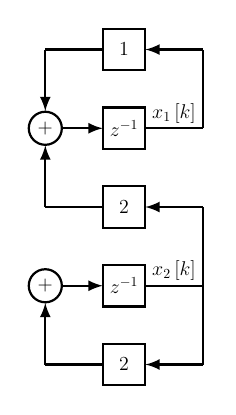
\begin{tikzpicture}[scale=0.5, transform shape, thick, node distance=2cm]
\draw
    node [input, name=input1] {} 
    node [sum, right of=input1] (suma1) {\suma}
    node [block, right of=suma1] (inte1) {{\Large $z^{-1}$}}
    node [output, right of=inte1, name=output1] {}
    node [block, above of=inte1] (scale11) {{\Large $1$}}
    node [input, right of=scale11, name=temp11] {}
    node [output, above of=suma1, name=temp12] {}

    node [block, below of=inte1] (scale12) {{\Large $2$}}
    node [input, left of=scale12, name=temp31] {}
    node [input, right of=scale12, name=temp32] {}

    node [sum, below of=temp31] (suma2) {\suma}
    node [input, left of=suma2, name=input2] {}
    node [block, right of=suma2] (inte2) {{\Large $z^{-1}$}}
    node [output, right of=inte2, name=output2] {}    
    node [block, below of=inte2] (scale22) {{\Large $2$}}
    node [input, right of=scale22, name=temp21] {}
    node [output, below of=suma2, name=temp22] {};

    % \draw[-latex](input1) -- node {}(suma1);
    \draw[-latex](suma1) -- node {} (inte1);
    \draw[-](inte1) -- node [above] {{\Large $x_1\dt{k}$}}(output1);
    \draw[-](output1) -- node {}(temp11);
    \draw[-latex](temp11) -- node {}(scale11);
    \draw[-](scale11) -- node {}(temp12);
    \draw[-latex](temp12) -- node {}(suma1);

    % \draw[-latex](input2) -- node {}(suma2);
    \draw[-latex](suma2) -- node {} (inte2);
    \draw[-](inte2) -- node [above] {{\Large $x_2\dt{k}$}}(output2);
    \draw[-](output2) -- node {}(temp21);
    \draw[-latex](temp21) -- node {}(scale22);
    \draw[-](scale22) -- node {}(temp22);
    \draw[-latex](temp22) -- node {}(suma2);
    % \draw[-](output) -- node {}(suma1);

    \draw[-](output2) -- node {}(temp32);
    \draw[-latex](temp32) -- node {}(scale12);
    \draw[-](scale12) -- node {}(temp31);
    \draw[-latex](temp31) -- node {}(suma1);
\end{tikzpicture}
\end{center}
\end{column}

\begin{column}{0.3\textwidth}
\end{column}
\begin{column}{0.4\textwidth}
\end{column}
\end{columns}
\end{frame}


\begin{frame}[t]{Diagonalization of a linear system}
\begin{columns}[t]
\begin{column}{0.3\textwidth}
When $\mf{A}$ is diagonalizable.
\[ \tilde{\mf{x}}\dt{k+1} = \bmx 1  & 0\\0 & 2\emx \tilde{\mf{x}}\dt{k} \]

\begin{center}
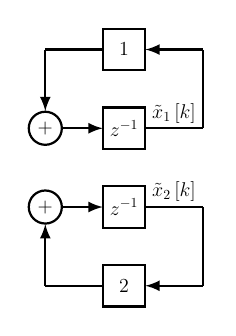
\begin{tikzpicture}[scale=0.5, transform shape, thick, node distance=2cm]
\draw
    node [input, name=input1] {} 
    node [sum, right of=input1] (suma1) {\suma}
    node [block, right of=suma1] (inte1) {{\Large $z^{-1}$}}
    node [output, right of=inte1, name=output1] {}    
    node [block, above of=inte1] (scale11) {{\Large $1$}}
    node [input, right of=scale11, name=temp11] {}
    node [output, above of=suma1, name=temp12] {}

    node [sum, below of=suma1] (suma2) {\suma}
    node [input, left of=suma2, name=input2] {}
    node [block, right of=suma2] (inte2) {{\Large $z^{-1}$}}
    node [output, right of=inte2, name=output2] {}    
    node [block, below of=inte2] (scale22) {{\Large $2$}}
    node [input, right of=scale22, name=temp21] {}
    node [output, below of=suma2, name=temp22] {};

    % \draw[-latex](input1) -- node {}(suma1);
    \draw[-latex](suma1) -- node {} (inte1);
    \draw[-](inte1) -- node [above] {{\Large $\tilde{x}_1\dt{k}$}}(output1);
    \draw[-](output1) -- node {}(temp11);
    \draw[-latex](temp11) -- node {}(scale11);
    \draw[-](scale11) -- node {}(temp12);
    \draw[-latex](temp12) -- node {}(suma1);

    % \draw[-latex](input2) -- node {}(suma2);
    \draw[-latex](suma2) -- node {} (inte2);
    \draw[-](inte2) -- node [above] {{\Large $\tilde{x}_2\dt{k}$}}(output2);
    \draw[-](output2) -- node {}(temp21);
    \draw[-latex](temp21) -- node {}(scale22);
    \draw[-](scale22) -- node {}(temp22);
    \draw[-latex](temp22) -- node {}(suma2);
    % \draw[-](output) -- node {}(suma1);
\end{tikzpicture}
\end{center}
\end{column}

\begin{column}{0.3\textwidth}
\end{column}
\begin{column}{0.4\textwidth}
\end{column}
\end{columns}
\end{frame}


\begin{frame}[t]{Diagonalization of a linear system}
\begin{columns}[t]
\begin{column}{0.4\textwidth}
When $\mf{A}$ is not-diagonalizable.
\[ \tilde{\mf{x}}\dt{k+1} = \bmx 1  & 1\\0 & 1\emx \tilde{\mf{x}}\dt{k} \]
\begin{center}
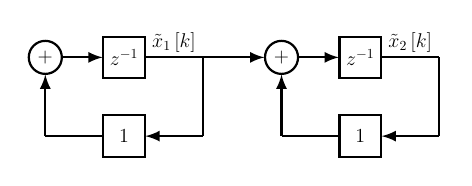
\begin{tikzpicture}[scale=0.5, transform shape, thick, node distance=2cm]
\draw
    node [input, name=input1] {} 
    node [sum, right of=input1] (suma1) {\suma}
    node [block, right of=suma1] (inte1) {{\Large $z^{-1}$}}
    node [output, right of=inte1, name=output1] {}    
    node [block, below of=inte1] (scale11) {{\Large $1$}}
    node [input, right of=scale11, name=temp11] {}
    node [output, below of=suma1, name=temp12] {}

    % node [input, right of=output1, name=input2] {}
    node [sum, right of=output1] (suma2) {\suma}
    node [block, right of=suma2] (inte2) {{\Large $z^{-1}$}}
    node [output, right of=inte2, name=output2] {}    
    node [block, below of=inte2] (scale22) {{\Large $1$}}
    node [input, right of=scale22, name=temp21] {}
    node [output, below of=suma2, name=temp22] {};

    % \draw[-latex](input1) -- node {}(suma1);
    \draw[-latex](suma1) -- node {} (inte1);
    \draw[-](inte1) -- node [above] {{\Large $\tilde{x}_1\dt{k}$}}(output1);
    \draw[-](output1) -- node {}(temp11);
    \draw[-latex](temp11) -- node {}(scale11);
    \draw[-](scale11) -- node {}(temp12);
    \draw[-latex](temp12) -- node {}(suma1);

    \draw[-latex](output1) -- node {}(suma2);
    \draw[-latex](suma2) -- node {} (inte2);
    \draw[-](inte2) -- node [above] {{\Large $\tilde{x}_2\dt{k}$}}(output2);
    \draw[-](output2) -- node {}(temp21);
    \draw[-latex](temp21) -- node {}(scale22);
    \draw[-](scale22) -- node {}(temp22);
    \draw[-latex](temp22) -- node {}(suma2);
\end{tikzpicture}
\end{center}
A Jordan block results in series of simple (scalar) first order blocks, where the output of a block acts as the input to another.
\end{column}

\begin{column}{0.3\textwidth}
\end{column}
\begin{column}{0.3\textwidth}
\end{column}
\end{columns}
\end{frame}


\begin{frame}[t]{Modes of a discrete-time system}
\vspace{-0.5cm}
\[ \mf{x}\dt{k} = \alpha_1 \lambda_1^k\mf{v}_1 + \alpha_2 \lambda_2^k\mf{v}_2 + \ldots + \alpha_n \lambda_n^k\mf{v}_n\]
\vspace{-0.5cm}

\begin{itemize}
    \item The eigvenvalues $\lc \lambda_i\rc_{i=1}^n$ of the system matrix $\mf{A}$ characterize the ``natural'' behavior of the system. These are called the \textit{modes of the system}.

    \item \textbf{Dominant mode}: Determines the long-term behavior of the system. In the case of discrete-time systems, this would be the eigenvalue with the largest magnitude.

    \item If $\lambda_i$ is a dominant mode $\implies \lv \alpha_i \lambda_i^k \rv \gg \lv \alpha_j \lambda_j^k \rv, \forall j \neq i$ and $k > N$.

    This implies that after some time, the response almost only has that particular mode,
    \[ \mf{x}\dt{k} \approx \alpha_i \lambda_i^k\mf{v}_i, \,\,\, \forall t > T \]

    \item \textbf{Subdominant mode}: These are the other modes of the system, and these essentially determine how fast the system moves to the dominant mode.
\end{itemize}
\end{frame}

\end{document}